%----------------------------------------------------------------------------------------
%	PACKAGES AND THEMES
%----------------------------------------------------------------------------------------

\documentclass{beamer}

\mode<presentation> {

% The Beamer class comes with a number of default slide themes
% which change the colors and layouts of slides. Below this is a list
% of all the themes, uncomment each in turn to see what they look like.

\usetheme{default}
%\usetheme{AnnArbor}
%\usetheme{Antibes}
%\usetheme{Bergen}
%\usetheme{Berkeley}
%\usetheme{Berlin}
%\usetheme{Boadilla} %<- I like this one
%\usetheme{CambridgeUS}
%\usetheme{Copenhagen}
%\usetheme{Darmstadt}
%\usetheme{Dresden}
%\usetheme{Frankfurt}
%\usetheme{Goettingen}
%\usetheme{Hannover}
%\usetheme{Ilmenau}
%\usetheme{JuanLesPins}
%\usetheme{Luebeck}
%\usetheme{Madrid}
%\usetheme{Malmoe}
%\usetheme{Marburg}
%\usetheme{Montpellier}
%\usetheme{PaloAlto}
%\usetheme{Pittsburgh}
%\usetheme{Rochester}
%\usetheme{Singapore}
%\usetheme{Szeged}
%\usetheme{Warsaw}

% As well as themes, the Beamer class has a number of color themes
% for any slide theme. Uncomment each of these in turn to see how it
% changes the colors of your current slide theme.

%\usecolortheme{albatross}
%\usecolortheme{beaver}
%\usecolortheme{beetle}
%\usecolortheme{crane}
%\usecolortheme{dolphin} %<- possibly -- a good simple blue
\usecolortheme{dove} %<- possibly -- all white
%\usecolortheme{fly}
%\usecolortheme{lily} 
%\usecolortheme{orchid} 
%\usecolortheme{rose} 
%\usecolortheme{seagull} %<- possibly -- a good simple gray
%\usecolortheme{seahorse}
%\usecolortheme{whale}
%\usecolortheme{wolverine}

%\setbeamertemplate{footline} % To remove the footer line in all slides uncomment this line
%\setbeamertemplate{footline}[page number] % To replace the footer line in all slides with a simple slide count uncomment this line

\setbeamertemplate{navigation symbols}{} % To remove the navigation symbols from the bottom of all slides uncomment this line

}
\setbeamertemplate{caption}[numbered]

\usepackage{graphicx} % Allows including images
\usepackage{booktabs} % Allows the use of \toprule, \midrule and \bottomrule in tables
\usepackage{bm, amsmath, amssymb, physics}
\usepackage{enumerate, enumitem}
\usepackage{multicol}
\usepackage{cancel}

\renewcommand*\footnoterule{}

%----------------------------------------------------------------------------------------
%	TITLE PAGE
%----------------------------------------------------------------------------------------

\title[Bias in MOT Estimation]{Quantifying the Bias in MOT Reconstruction from Noble Gas Saturation Anamolies between the LGM and PI} % The short title appears at the bottom of every slide, the full title is only on the title page

\author[Perrin W. Davidson]{Perrin Davidson\inst{1, 2} \and Alan Seltzer\inst{1} \and David Nicholson\inst{1} \and Samar Khatiwala\inst{3} \and Sarah Shackleton\inst{4}} % Authors

\institute[MIT-WHOI]{
  \inst{1}%
  Department of Marine Chemistry and Geochemistry\\
  Woods Hole Oceanographic Institution
  \and
  \inst{2}%
  Earth, Atmospheric, and Planetary Sciences\\
  Massachusetts Institute of Technology
  \and
  \inst{3}%
  Department of Earth Sciences\\
  University of Oxford
  \and
  \inst{4}%
  Department of Geosciences\\
  Princeton University
} % Institutions

\date[]{\today} % Date

\begin{document}

\begin{frame}
\titlepage % Print the title page as the first slide
\end{frame}

%----------------------------------------------------------------------------------------
%	PRESENTATION SLIDES
%----------------------------------------------------------------------------------------

%------------------------------------------------
\section{Where are we now?} 
%------------------------------------------------

%------------------------
\begin{frame}
    \vfill
    \centering
    \begin{beamercolorbox}[sep=8pt,center,shadow=false,rounded=false]{title}
        \usebeamerfont{title}
        \insertsectionhead
        \par
    \end{beamercolorbox}
    \vfill
\end{frame}
%------------------------

%------------------------
\begin{frame}
\frametitle{A Brief Overview}

\begin{itemize}
	\item We couple a gas exchange model with an ESCM to estimate the global, volume-weighted mean $\Delta$ of the following gases: N$_2$, Ne, Ar, Kr, and Xe. 
	\item The bubble flux model parameterizes flux via the simplified following equation:
		\begin{equation}
			\mathcal{F}_n = \mathcal{F}_s + \mathcal{F}_p + \mathcal{F}_c \propto u_{10}^l,
		\end{equation}
		for $l$ a range of power laws presented in \emph{Liang et al. (2013)}.
	\item This suggests that while there are many parameter sensitivities to test, the effect of changing winds are to leading order the most important to gain an understanding of.
\end{itemize}

\end{frame}
%------------------------

%------------------------
\begin{frame}
% \frametitle{Title}
% \framesubtitle{Subtitle} 
	\begin{figure}
        	\centering
        	\vfill
		\includegraphics[width=\textwidth]{images/1}
        	\label{fig:1}
        	\vfill
    	\end{figure}    
\end{frame}
%------------------------

%------------------------
\begin{frame}
% \frametitle{Title}
% \framesubtitle{Subtitle} 
	\begin{figure}
        	\centering
		\vfill
        	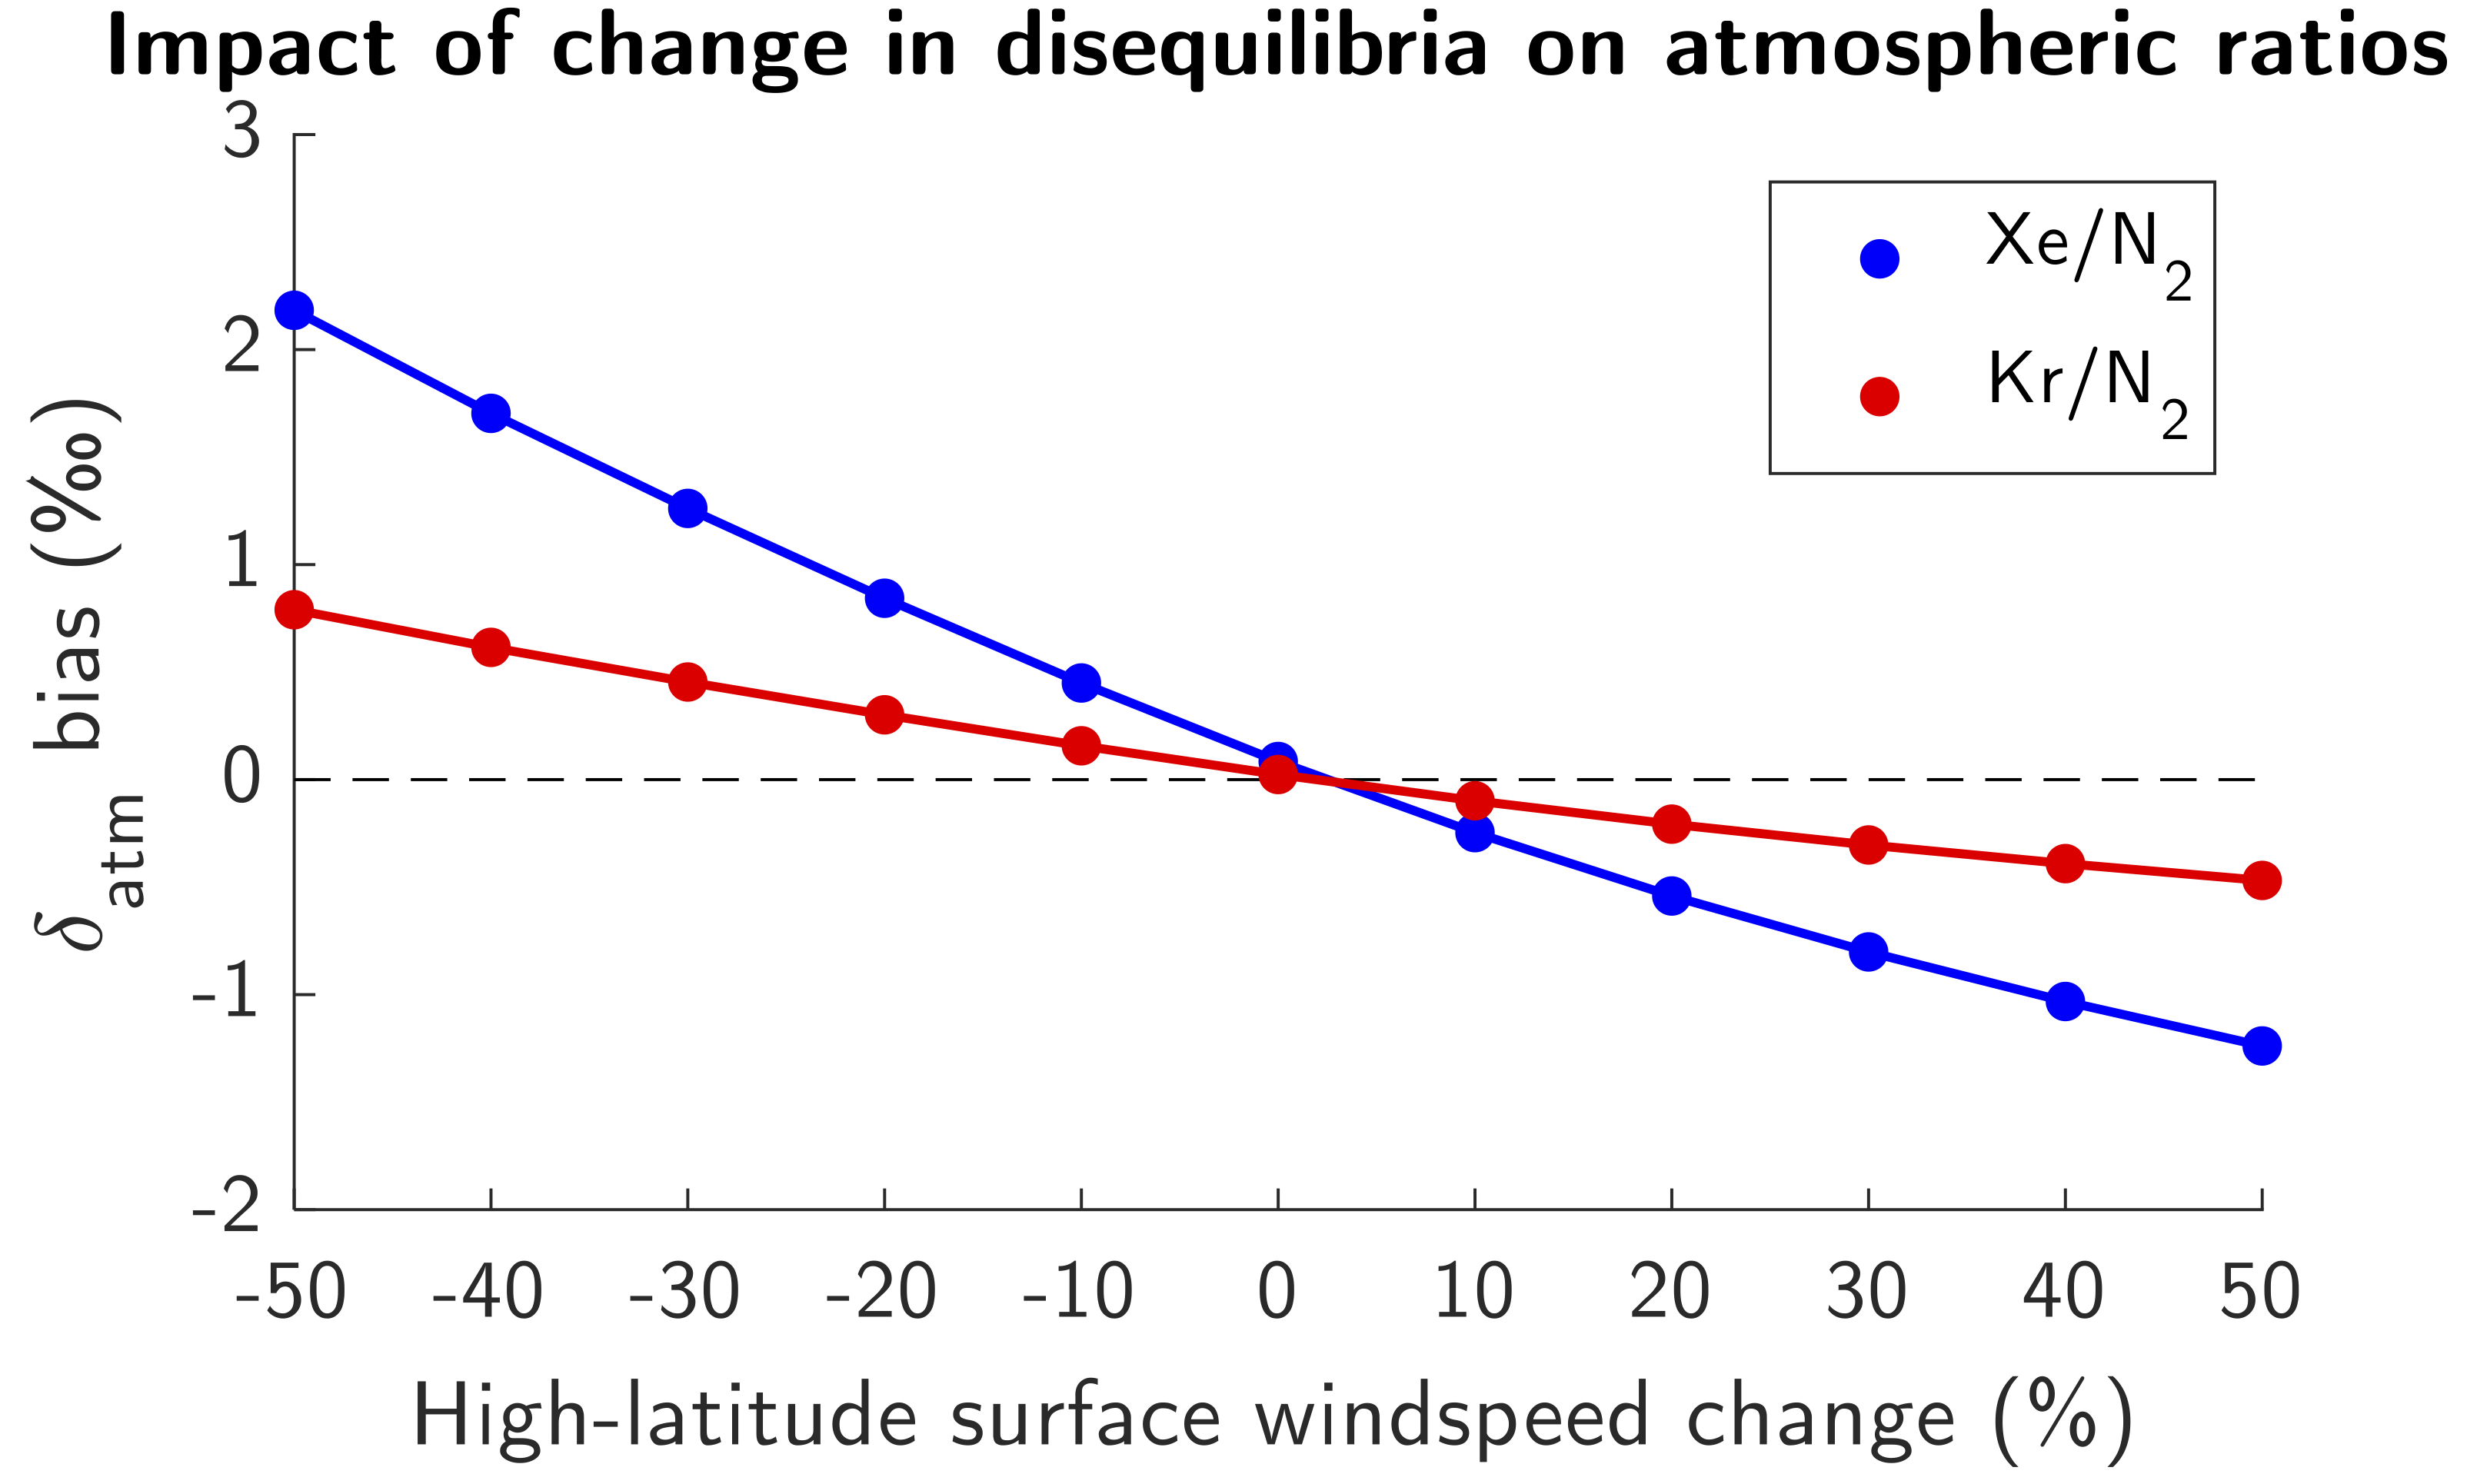
\includegraphics[width=\textwidth]{images/2}
        	\label{fig:2}
        	\vfill
    	\end{figure}    
\end{frame}
%------------------------

%------------------------
\begin{frame}
% \frametitle{Title}
% \framesubtitle{Subtitle} 
	\begin{figure}
        	\centering
		\vfill
        	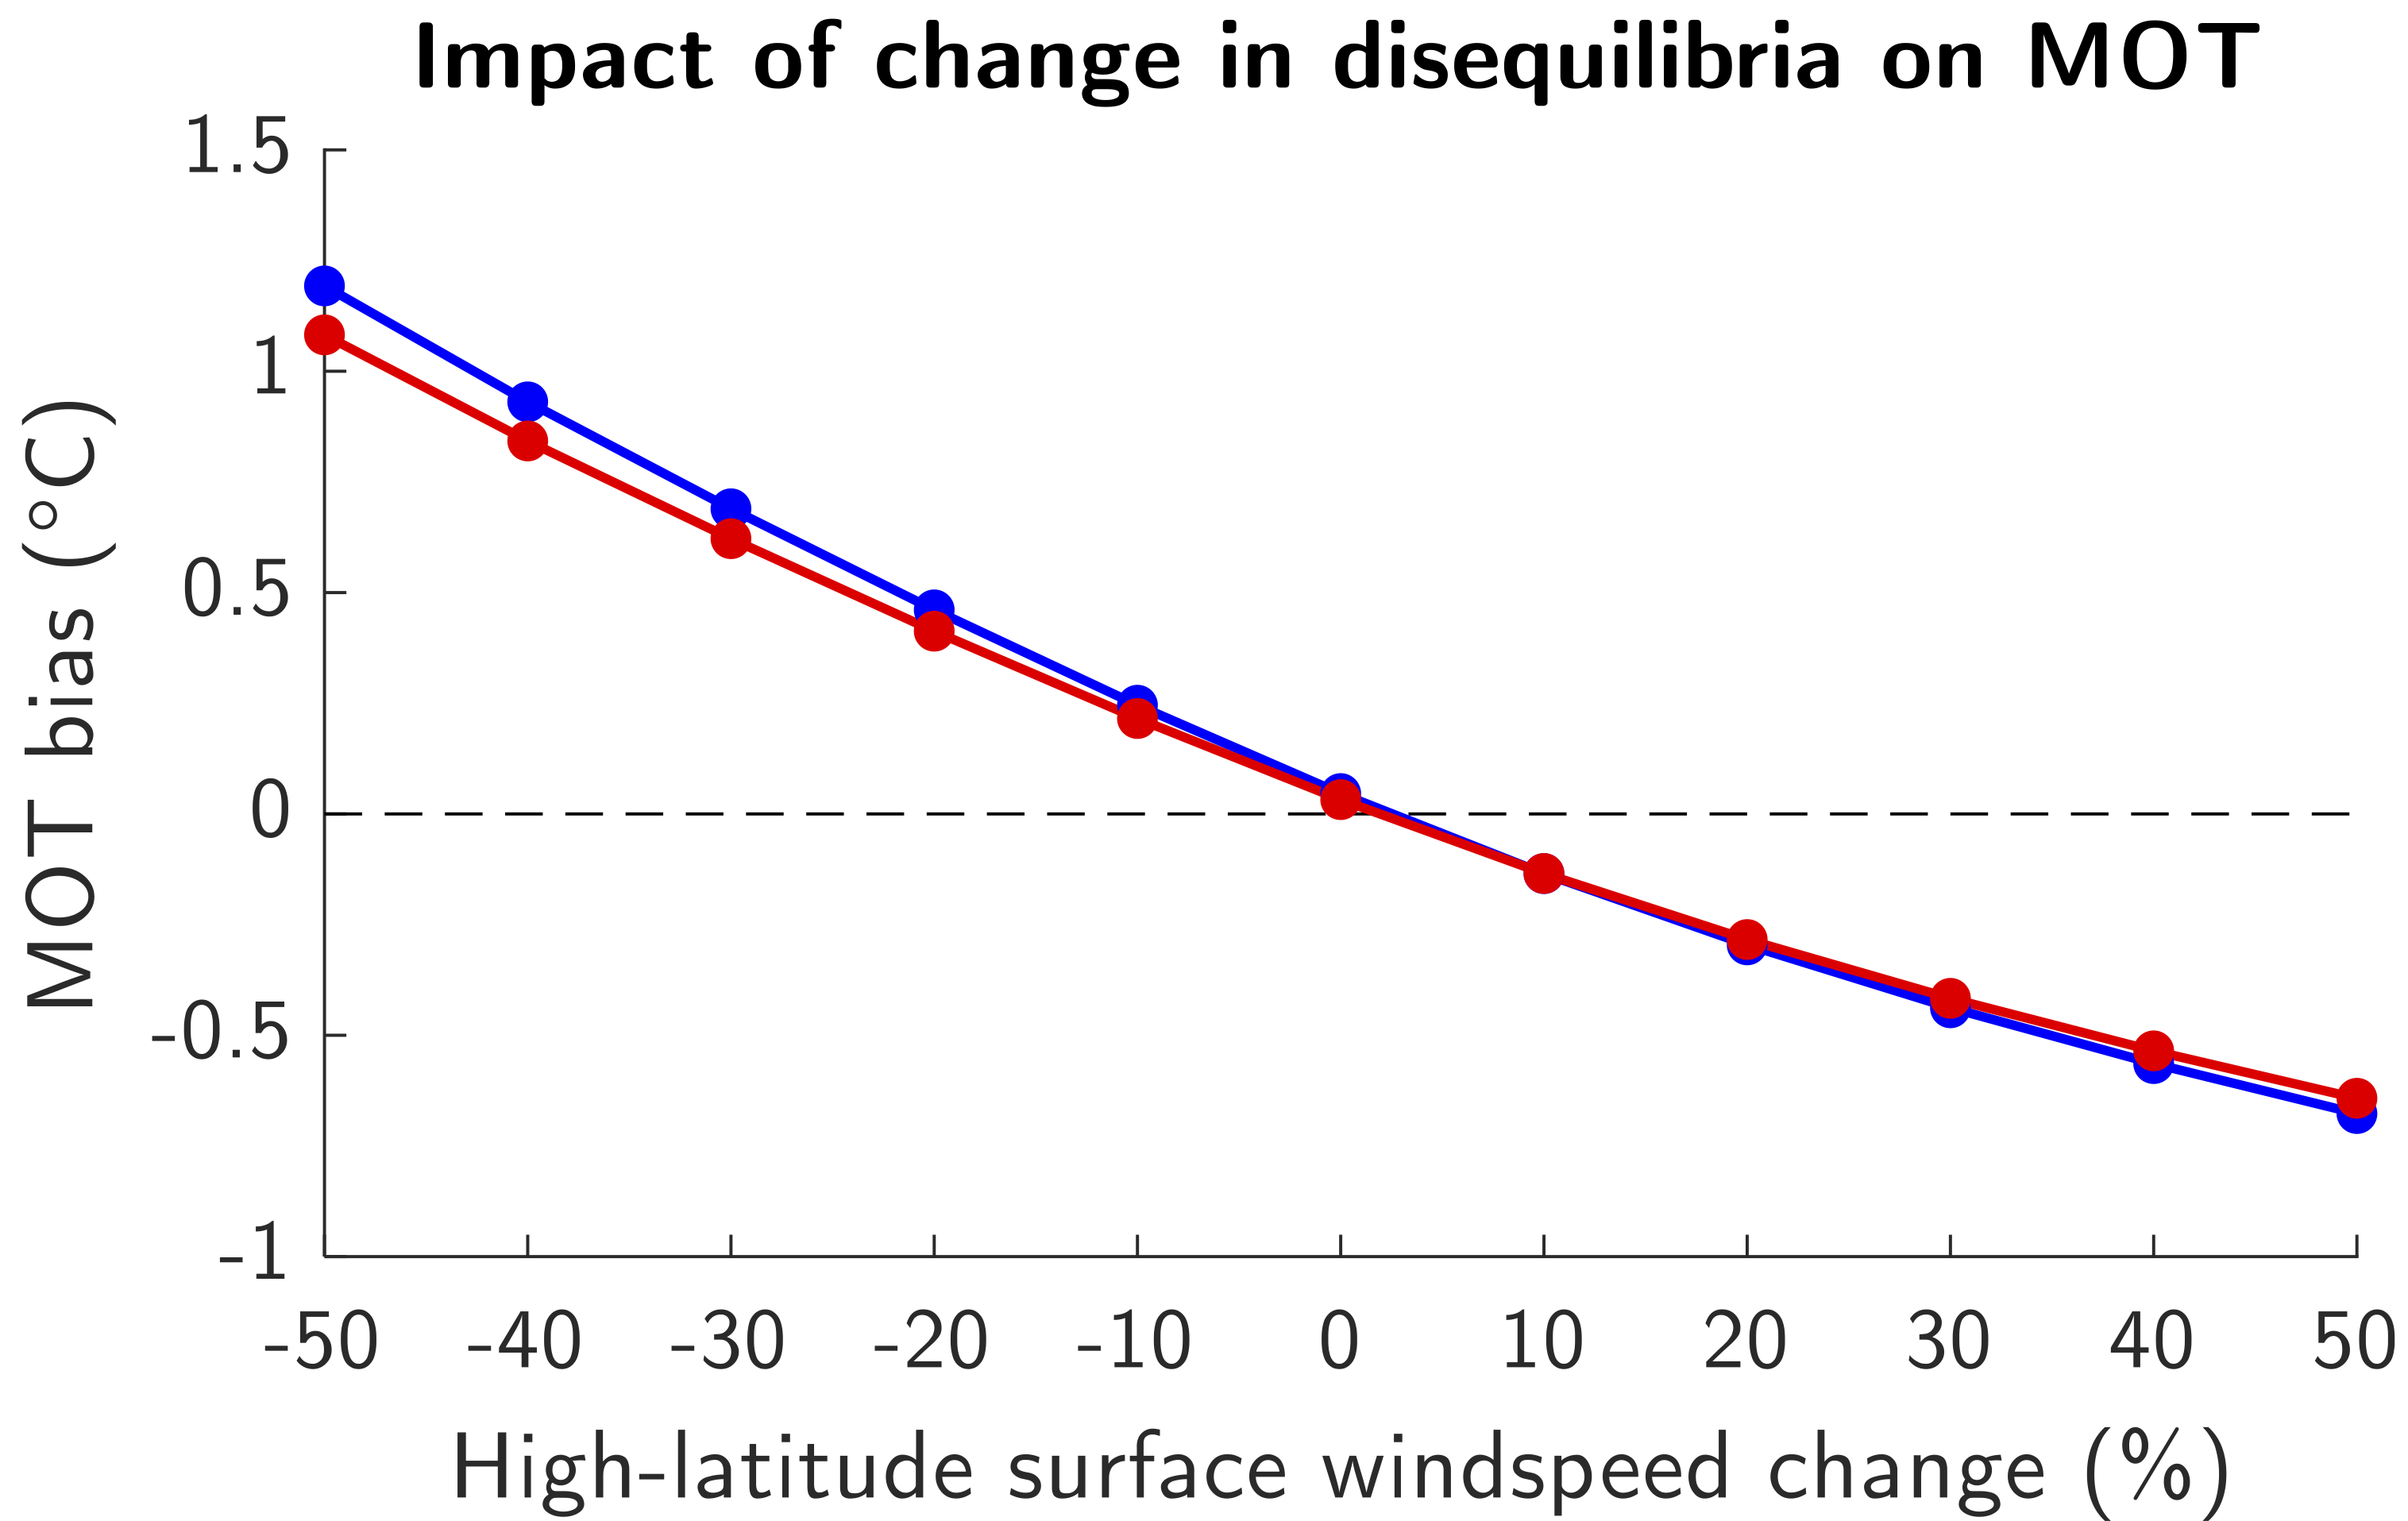
\includegraphics[width=\textwidth]{images/3}
        	\label{fig:3}
        	\vfill
    	\end{figure}    
\end{frame}
%------------------------

%------------------------
\begin{frame}
% \frametitle{Title}
% \framesubtitle{Subtitle} 
	\begin{figure}
        	\centering
		\vfill
        	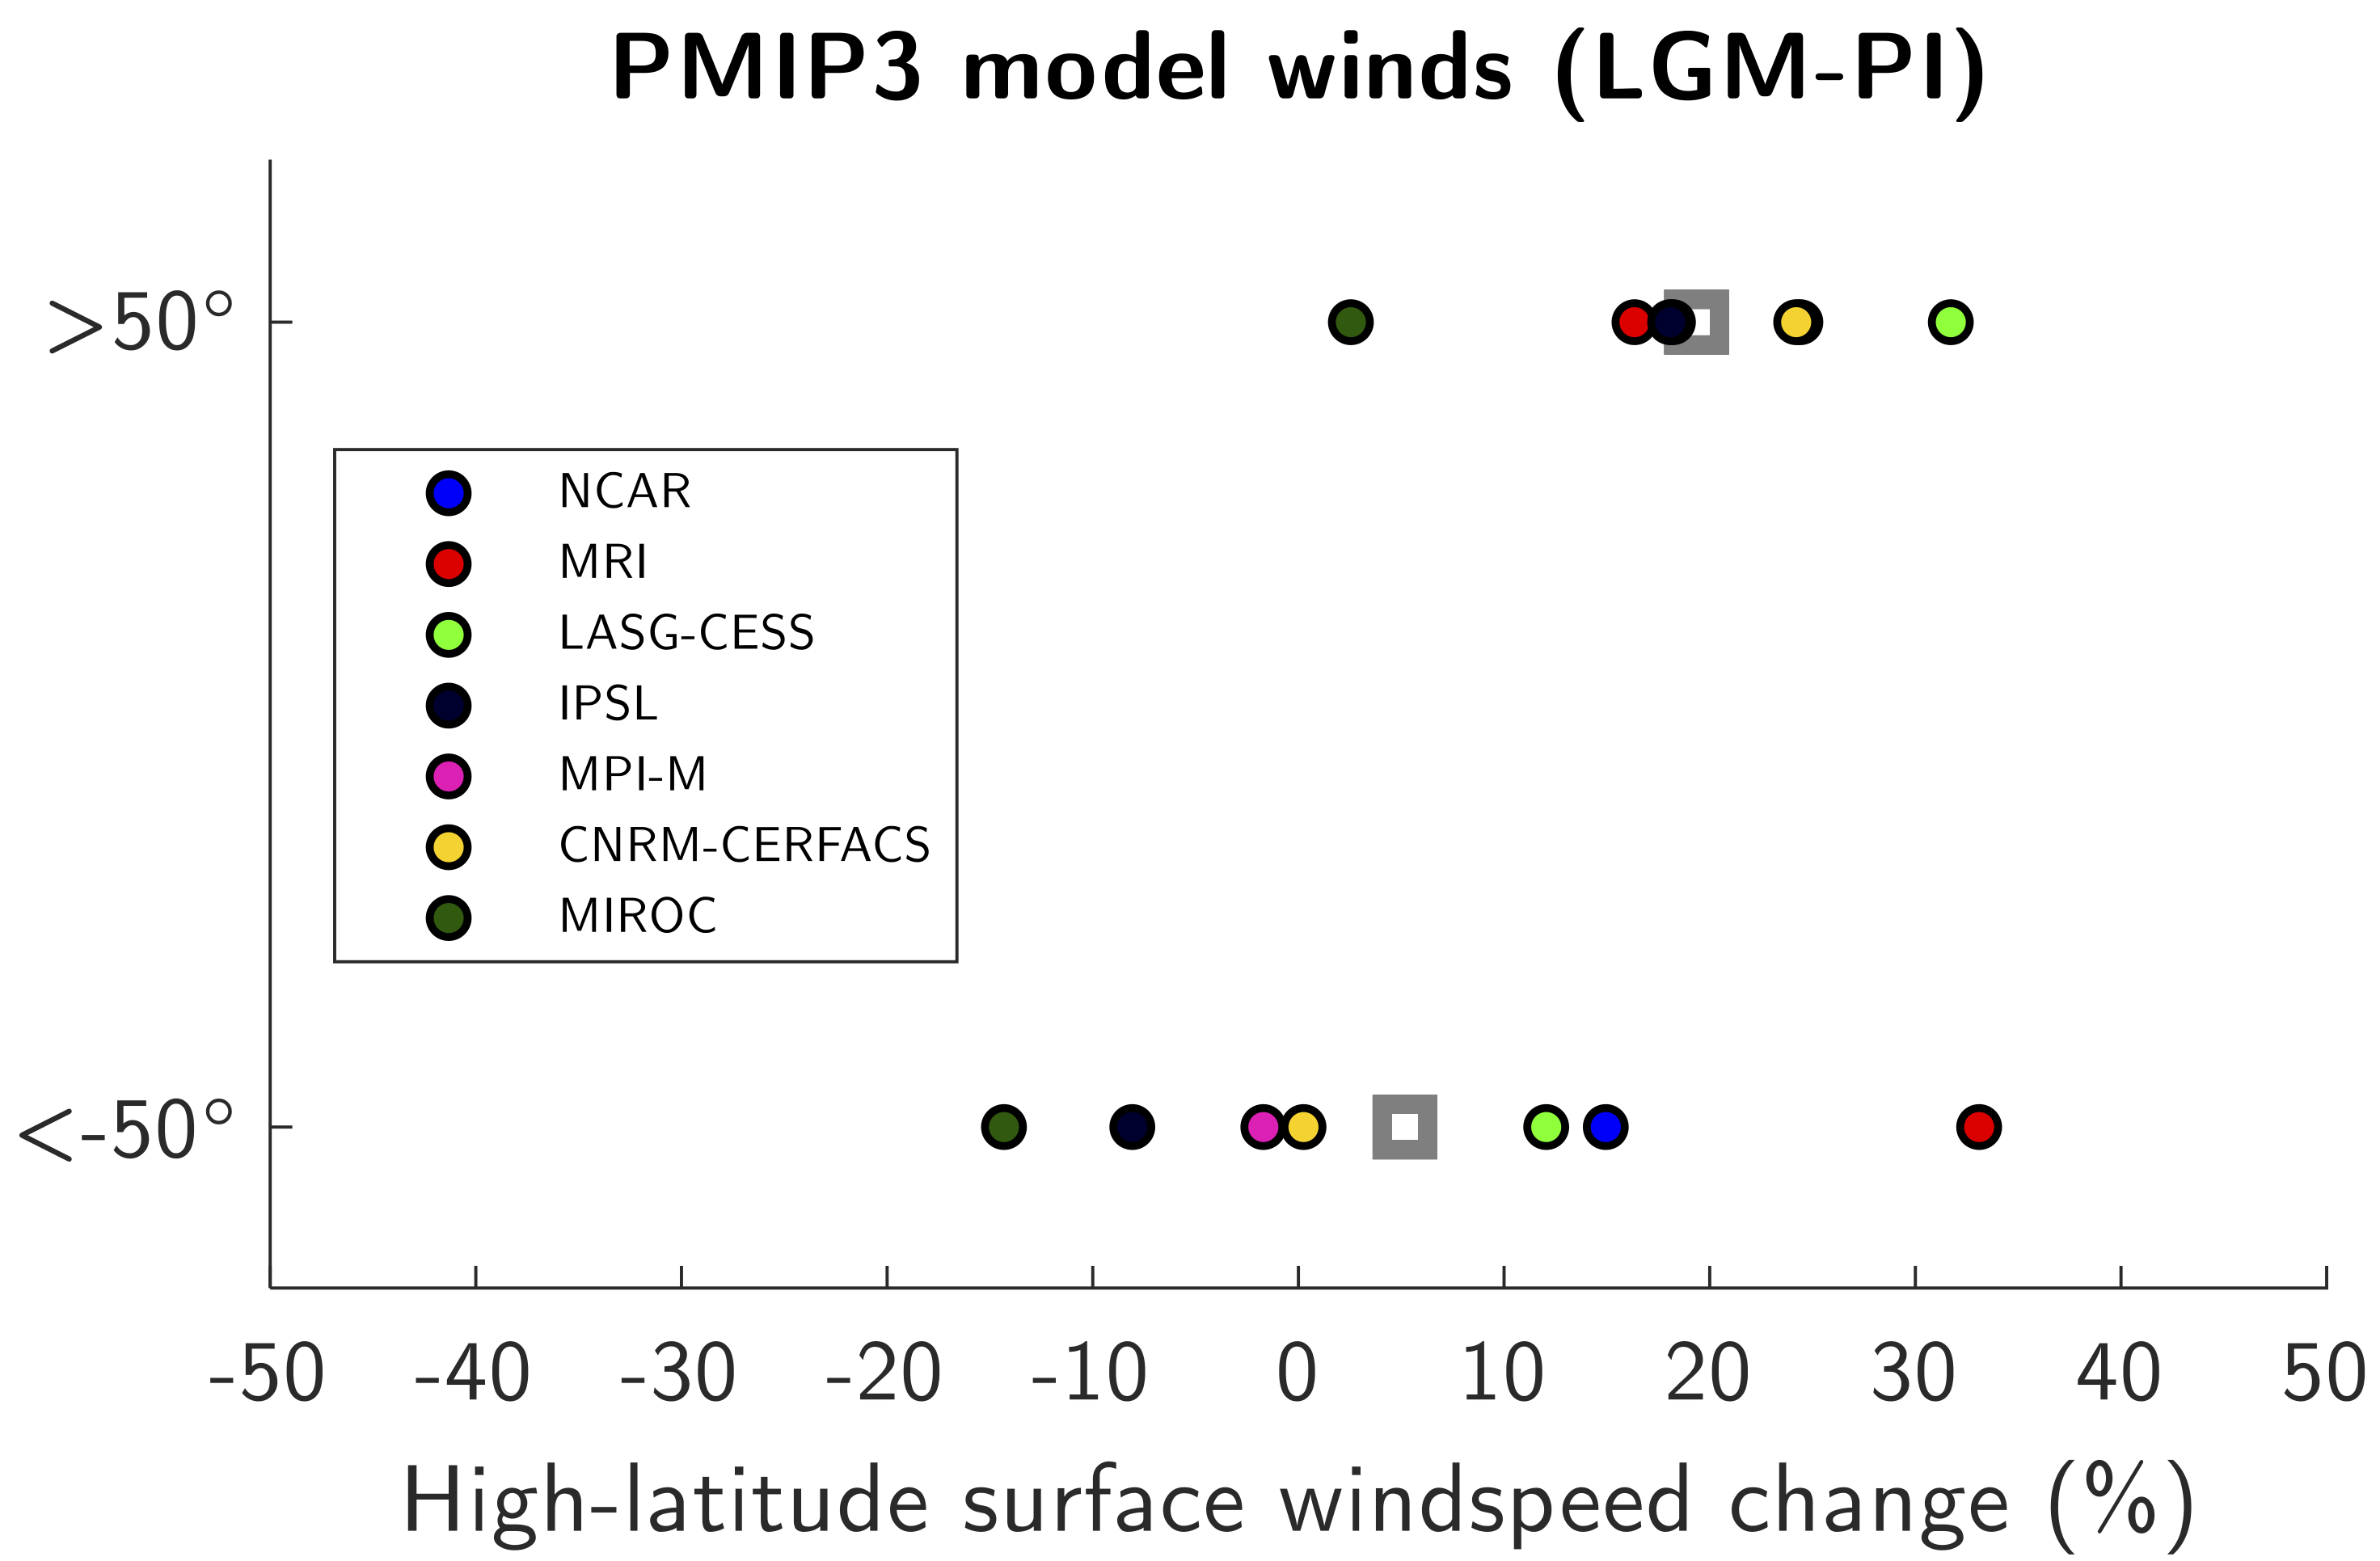
\includegraphics[width=\textwidth]{images/4}
        	\label{fig:4}
        	\vfill
    	\end{figure}    
\end{frame}
%------------------------

%------------------------
\begin{frame}
\frametitle{Bias Estimates}
From this work, we find the following bias in MOT reconstruction from Noble gas saturation anamolies:
\begin{table}
	\centering
	\begin{tabular}{c|c}
		\textbf{Windspeed (\%)} & \textbf{Bias ($^\circ$C)} \\
		\hline
		[0, +30] & [+0.05, -0.44] \\
	\end{tabular}
\end{table}
\end{frame}
%------------------------

%------------------------------------------------
\section{Where do we want to go?} 
%------------------------------------------------

%------------------------
\begin{frame}
    \vfill
    \centering
    \begin{beamercolorbox}[sep=8pt,center,shadow=false,rounded=false]{title}
        \usebeamerfont{title}
        \insertsectionhead
        \par
    \end{beamercolorbox}
    \vfill
\end{frame}
%------------------------

%------------------------
\begin{frame}
\frametitle{Next Steps}

Some possible new directions: \par\vspace{0.2cm}

\begin{itemize}
	\item 1.) Run these simulations with the ECCO or mitGCM-derived TMs,
	\item 2.) Develop a simple, dynamical model of bubble evolution in the surface ocean to better understand the mechanisms behind the parameterizations from \emph{Liang et al. (2013)},
	\item 3.) Work on sub-grid scale parameterizations derived from probability density functions of parameters and extreme value theory (i.e., committor probability).
\end{itemize}

\end{frame}
%------------------------

\end{document}

%----------------------------------------------------------------------------------------
